% (c) 2012 - 2014 - Dimitrios Vrettos d.vrettos@gmail.com
\section{Esercizi}

\subsection{Esercizi dei singoli paragrafi}

\subsubsection*{E.1.1 - La costruzione dell'insieme dei numeri interi relativi}

\begin{esercizio}
\label{ese:E.1}
Completa la tabella secondo le definizioni di numero intero relativo fornite nella sezione~\ref{sect:ins_numeri_interi_relativi} a pagina~\pageref{sect:ins_numeri_interi_relativi}.
\begin {center}
\begin{tabular}{ccc}
 \toprule
  Intero relativo & Elementi classe equivalenza & Forma canonica\\
  $[(5;7)]$ & & \\
   & $(7;5)$, $(11;9)$, $(34;32)$, $(3;1)$, $\dotfill$ & \\
   & & $(7;0)$\\
  $[(56;90)]$ & & \\
   & $(3;3)$, $(76;76)$, $(9;9)$, $(43;43)$, \ldots & \\
   & & $(0;4)$\\
   & $(4;9)$, $(8;13)$, $(57;62)$, $\dotfill$ & \\
  \bottomrule
 \end{tabular}
\end{center}
\end{esercizio}

\begin{esercizio}
\label{ese:E.2}
Completa la tabella secondo le definizioni di numero intero relativo fornite nella sezione~\ref{sect:ins_numeri_interi_relativi} a pagina~\pageref{sect:ins_numeri_interi_relativi}.
\begin {center}
\begin{tabular}{cccc}
 \toprule
  Intero relativo & Forma canonica & Simbolo usuale & Valore assoluto\\
   & &$+6$& \\
   &$(0;2)$& & \\
  $[(5;5)]$& & & \\
   & &$-1$& \\
  \bottomrule
 \end{tabular}
\end{center}
\end{esercizio}

\subsubsection*{E.1.2 - La costruzione dell'insieme dei numeri razionali}
\begin{esercizio}
\label{ese:E.3}
Secondo le definizioni di numero razionale fornite nella sezione~\ref{sect:ins_numeri_razionali} a pagina~\pageref{sect:ins_numeri_razionali},
completa il ragionamento: alla coppia~$(6;4)$ viene associata la frazione \ldots; alla coppia~$(\ldots; \ldots)$ è associata
la frazione~$\frac{3}{2}$. Le coppie \ldots\ldots stanno nella \ldots\ldots;
le frazioni \ldots\ldots sono equivalenti secondo l'usuale definizione.
\end{esercizio}

\begin{esercizio}
\label{ese:E.4}
Ripeti l'esercizio precedente prendendo coppie di~$\insN \times \insN_0$ in relazione tra loro e mostrando che la relazione è di equivalenza tra le rispettive frazioni.
\end{esercizio}

\begin{esercizio}
\label{ese:E.5}
Completa la catena di trasformazioni.
\begin {center}
\begin{tabular}{ccc}
 \toprule
  Coppie & Razionale come frazione & Razionale come decimale\\
  $(1;2)\,\Rel\,(3;6)$&$\frac{1}{2}$&$\np{0,5}$\\
  $(2;7)\,\Rel\,(4;49)$& & \\
  $(8;5)\,\Rel\,(40;25)$& & \\
  $(60;12)\,\Rel\,(10;2)$& & \\
  $(2;3)\,\Rel\,(12;18)$& & \\
  \bottomrule
 \end{tabular}
\end{center}
\end{esercizio}

\subsubsection*{E.1.3 - Classi resto modulo~$7$}
\begin{esercizio}
\label{ese:E.6}
Determina gli elementi di~$\insN_7$.

Nell'insieme~$\insN$ si considera la relazione d'equivalenza~$\Rel$:
``avere lo stesso resto nella divisone per~$7$''. Le classi d'equivalenza sono:~$[0], [\ldots], \ldots, [6]$.
Nella classe~$[0]$ stanno tutti i \ldots\ldots che divisi per~7 danno \ldots, cioè \dotfill.
In quale classe sta il numero~$427$? E il numero~$74$?
\end{esercizio}

\begin{esercizio}
\label{ese:E.7}
Nell'insieme~$\insZ_6$ delle classi di resto modulo~$6$ si può definire la somma e il prodotto ricalcandole dall'addizione e moltiplicazione
dei numeri naturali. Si ha pertanto:~$[1]+[2]=[3]$, $[4]+[5]=[3]$ infatti~$4+5=9$ ma~$[9]=[3]$.

Determina:~$[5]+[3]=[\ldots]$; $[3]+[3]=[\ldots]$; $[1]+[0]=[\ldots]$.

Analogamente si può definire la moltiplicazione:~$[5]\cdot [3]=[3]$
infatti~$5\cdot 3=15$ ma~$15:6=2$ con il resto di~$3$, quindi \dotfill

Determina:~$[5]\cdot [2]=[\ldots]$, $[3]\cdot [1]=[\ldots]$, $[3]\cdot [0]=[\ldots]$.
\end{esercizio}

\begin{esercizio}
\label{ese:E.8}
In maniera analoga a quanto è stato definito con $\insN_n$ è possibile estendere il concetto anche a $\insZ_n$. Elenca e descrivi gli elementi dell'insieme~$Z_{12}$.

Trovi qualche analogia con il disegno dell'orologio riprodotto nella figura~\ref{fig:E.10}?
Come rispondi alla domanda: ``quale numero indica la lancetta delle ore $5$ ore dopo le~$9$ di mattina?''
\`E sbagliato dire ``$4$ ore dopo le~$9$ di mattina sono le~$2$''?
\end{esercizio}

\begin{esercizio}
\label{ese:E.9}
Al banco della frutta e verdura del supermercato la bilancia presenta una tastiera come quella nella figura~\ref{fig:E.11}.
Premendo il bottone relativo alla frutta da pesare si ottiene l'adesivo con il prezzo.
Sistema, senza contare casella per casella, il numero che corrisponde ai miei acquisti di oggi:
zucchine al numero~$75$, arance al numero~$63$, spinaci al numero~$48$, patate al numero~$56$.
Hai potuto sfruttare le classi di resti modulo~$8$?
\end{esercizio}

\begin{figure}[hb]
 \begin{minipage}[t]{.45\textwidth}
 \centering% (c) 2012 Dimitrios Vrettos - d.vrettos@gmail.com
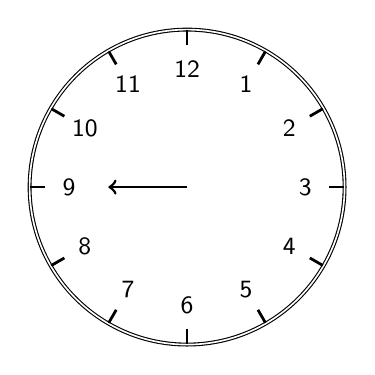
\begin{tikzpicture}[font=\small,x=6mm,y=6mm]
    \draw [double] (0,0) circle (2cm);
    \foreach \angle/ \label in{0/3, 30/2, 60/1, 90/12, 120/11, 150/10, 180/9,210/8, 240/7, 270/6, 300/5, 330/4}
    {
      \draw[line width=1pt] (\angle:1.8cm) -- (\angle:1.99cm);
      \draw (\angle:1.5cm) node{\textsf{\label}};
    }
      \draw[->,line width=1pt] (0,0) -- (180:1cm);
\end{tikzpicture}
 \caption{Esercizio~\ref{ese:E.8}.}\label{fig:E.10}
 \end{minipage}\hfil
 \begin{minipage}[t]{.45\textwidth}
 \centering% (c) 2012 Dimitrios Vrettos - d.vrettos@gmail.com
\begin{tikzpicture}[x=6mm,  y=6mm]
  \newcounter{num}
  \setcounter{num}{0}
  
  \draw[color=gray, step=6mm] (0,0) grid (8,10);
  \foreach \y in {9,8,...,0}{
    \foreach \x in {0,1,...,7}{
      \stepcounter{num}
      \ifnum \thenum<28
	\draw[xshift=3mm,yshift=3mm] (\x , \y ) node {\thenum};
      \fi
    }
  }
  
  \foreach \j in {10,9,8,...,0}
    \foreach \i in {0,1,...,8}
      \draw[] (\i , \j ) node[fill=white] {};
\end{tikzpicture}
 \caption{Esercizio~\ref{ese:E.9}.}\label{fig:E.11}
 \end{minipage}
\end{figure}


\subsubsection*{E.2 - Insiemi finiti e insiemi infiniti}

\begin{esercizio}
\label{ese:E.10}
Stabilisci la cardinalità dell'insieme~$V$ delle vocali della lingua italiana e dell'insieme~$D$ delle dita di una mano.

Completa l'insieme~$V$.

\`E possibile stabilire una corrispondenza biunivoca tra $V$ e $D$? Se sì, descrivila con una tabella.

Determina~$\insN_{5}$: \dotfill

Cosa si può dire sulla cardinalità di $V$, $D$ e $\insN_5$?
\end{esercizio}

\begin{esercizio}
\label{ese:E.11}
Negli insiemi ``infiniti'' non possiamo affermare che ``la parte è minore del tutto''.

Prolungate i lati obliqui
del trapezio~${ABCD}$ rappresentato nella figura~\ref{fig:E.12} fino a farli incontrare nel punto~$O$.
Le semirette di origine~$O$ e comprese tra~${OA}$ e~${OB}$, proiettano il segmento~${DC}$ sul segmento~${AB}$,
facendo così corrispondere ad un ogni punto di~${DC}$ un punto di~${AB}$.
Direste vera o falsa l'affermazione: <<i punti del segmento~${DC}$ sono tanti quanti quelli del segmento~${AB}$>>?

Seguite questi passaggi rispondendo ai quesiti:
\begin{enumeratea}
 \item quale punto di~$AB$ corrisponde a~$D$? e quale a~$C$?
 \item ogni punto di~${CD}$ trova un corrispondente punto in~${AB}$?
 \item di quale punto di~$DC$ è immagine il punto~$K$ di~${AB}$?
 \item ogni punto di~${AB}$ è immagine di un solo punto di~${CD}$?
 \item la proiezione costruita stabilisce una corrispondenza biunivoca tra~${CD}$ e~${AB}$?
 \item a quale conclusione vi ha condotto questo esercizio?
\end{enumeratea}
\end{esercizio}
\begin{figure}[htb]
  \centering% (c) 2012 Dimitrios Vrettos - d.vrettos@gmail.com
\begin{tikzpicture}[x=8mm, y=8mm]
\tkzDefPoint(0,0){A}
\tkzDefPoint(7,0){B}
\tkzDefPoint(4,3){C}
\tkzDefPoint(1,3){D}
\tkzDefPoint(4,0){K}

\tkzDrawPolygon(A, B, C, D)

\tkzLabelPoints[below](A, B, K)
\tkzLabelPoints[above](C, D)

\tkzSetUpPoint[fill=CornflowerBlue,size=6]
\tkzDrawPoints(A, B, C, D, K)

\end{tikzpicture}
 \caption{Esercizio~\ref{ese:E.11}.}\label{fig:E.12}
\end{figure}


\begin{esercizio}
\label{ese:E.12}
Gli insiemi~$A=\{x\mid x=2n^{2}-1$ con~$n\in \insN$ e~$0\le n<2\}$ e~$B=\{y\in \insZ\mid -1\le y\le 1\}$
si possono mettere in corrispondenza biunivoca?
\end{esercizio}

\begin{esercizio}
\label{ese:E.13}
Dato l'insieme~$K=\{$a, b, c, d$\}$, costruite l'insieme~$K\times K$.
Considerate il suo sottoinsieme~$H=\{(x;y)\in K\times K \mid x\text{ precede }y\text{ nell'ordine alfabetico}\}$.
\`E vero che tale insieme è equipotente all'insieme formato dalle facce di un cubo?
\end{esercizio}

\begin{esercizio}
\label{ese:E.14}
Attraverso la costruzione di un grafo sagittale, attribuite il valore di verità alla proposizione: ``il sottoinsieme~$T$ di
$\insN\times \insN$ formato dalle coppie i cui elementi danno come somma~$3$ è equipotente all'insieme~$F$ dei divisori di~$14$''.
\end{esercizio}

\begin{esercizio}
\label{ese:E.15}
\TabPositions{12cm}
Attribuite il valore di verità alle seguenti proposizioni:
 \begin{enumeratea}
\item un insieme infinito è sempre numerabile \tab\boxV\quad\boxF
\item un insieme infinito può essere equipotente a un suo sottoinsieme proprio \tab\boxV\quad\boxF
\item la cardinalità dell'insieme~$\insQ$ è maggiore di quella dell'insieme~$\insZ$ \tab\boxV\quad\boxF
\item due insiemi equipotenti sono infiniti \tab\boxV\quad\boxF
\end{enumeratea}
\end{esercizio}

\begin{esercizio}
\label{ese:E.16}

Considerando l'insieme~$P=\left\{2^{n}\text{ con }n\in \insN\right\}$ delle potenze di~$2$,
completa la tabella sottostante:
\begin{center}
 \begin{tabular}{cccccccccccc}
  \toprule
  $n$ & $0$ & $1$ & $2$ & $3$ & $4$ & $5$ & $6$ & $7$ & $8$ & $9$ & $\cdots$\\
  $2^n$ & $1$ & $2$ & & & & & & & & & $\cdots$ \\
  \bottomrule
 \end{tabular}
\end{center}

Qual è il valore di verità delle seguenti proposizioni?
\begin{enumeratea}
\TabPositions{8cm}
\item $P$ è un sottoinsieme di~$\insN$ \tab\boxV\quad\boxF
\item $0 \in P$ \tab\boxV\quad\boxF
\item $P$ è numerabile \tab\boxV\quad\boxF
\item nessun elemento di~$P$ è maggiore di~$\np{2065438}$\tab\boxV\quad\boxF
\end{enumeratea}

Quali considerazioni potete fare sull'infinità di~$P$?
\end{esercizio}

\subsubsection*{E.3 - Strutture algebriche}

\begin{esercizio}
\label{ese:E.17}
Rispondete ai seguenti quesiti:
\begin{enumeratea}
\item Cos'è una struttura algebrica?
\item Con quale scrittura la si rappresenta?
\item L'insieme $A=\{$1, 2, 3, 4, 5, 6, 7, 8, 9, 10$\}$ con l'operazione di addizione è una struttura algebrica? Perché?
\item L'insieme $P=\{x\in\insN\mid x$ è pari$\}$ con l'operazione di addizione è una struttura algebrica? Perché? E con l'operazione di moltiplicazione?
\item L'insieme $N_5=\{$0, 1, 2, 3, 4$\}$ con l'operazione di modulo (resto intero della divisione) è una struttura algebrica? Perché?
\end{enumeratea}
\end{esercizio}

\begin{esercizio}
\label{ese:E.18}
Dimostrare che $(\insQ$, $\star)$ con $a \star b=ab−a−b+2$ è un monoide.

\emph{Suggerimento:} L'operazione $\star$ è interna a $\insQ$? Gode della proprietà associativa? Qual è l'elemento neutro?
\end{esercizio}

\begin{esercizio}
\label{ese:E.19}
Dimostrare che $(\insZ$, $-$, $\cdot)$ è un anello commutativo con
identità e integro.
\end{esercizio}

\begin{esercizio}
\label{ese:E.20}
Dimostrare che $(\insR$, $+$, $\cdot)$ è un campo.
\end{esercizio}
